\chapter{Rechenbefehle und Scripting im Warteschlangensimulator}

\renewcommand{\thepage}{\arabic{page}}
\setcounter{page}{1}

\textbf{Rechenbefehle} können im Simulator verwendet werden, um z.B.\ Zeitdauern
(wie Bedienzeiten) zu bestimmen oder um festzulegen, in welche
Verzweigungsrichtung ein Kunde geleitet werden soll.

Sowohl zur Bestimmung von Verzweigungsrichtungen aus auch bei der Auswertung von
Simulationsergebnissen und bei der Durchführung von Parameterreihen können
\textbf{Skripte} eingesetzt werden. Der Warteschlangensimulator verwendet dabei
als Sprachen Javascript und Java.

\section{Ausdrücke erstellen}

Rechts neben allen Eingabefeldern, in die ein Rechenbefehl eingegeben werden kann, ist
stets eine Schaltfläche mit dem folgenden Symbol zu sehen:
\fbox{
\includegraphics[width=0.25cm]{wand.png}}
Über diese Schaltfläche kann der \textbf{Ausdruck bearbeiten} Dialog
(siehe Abbildung \ref{fig:ExpressionBuilder}) aufgerufen werden.
Der Dialog enthält eine vollständige Liste aller im aktuellen Kontext zur Verfügung
stehenden Befehle und ermöglicht das einfache zusammenstellen komplexerer Befehle und
Ausdrücke.

\begin{figure}[ht]	
	\caption{,,Ausdruck bearbeiten''-Dialog}
	\centerline{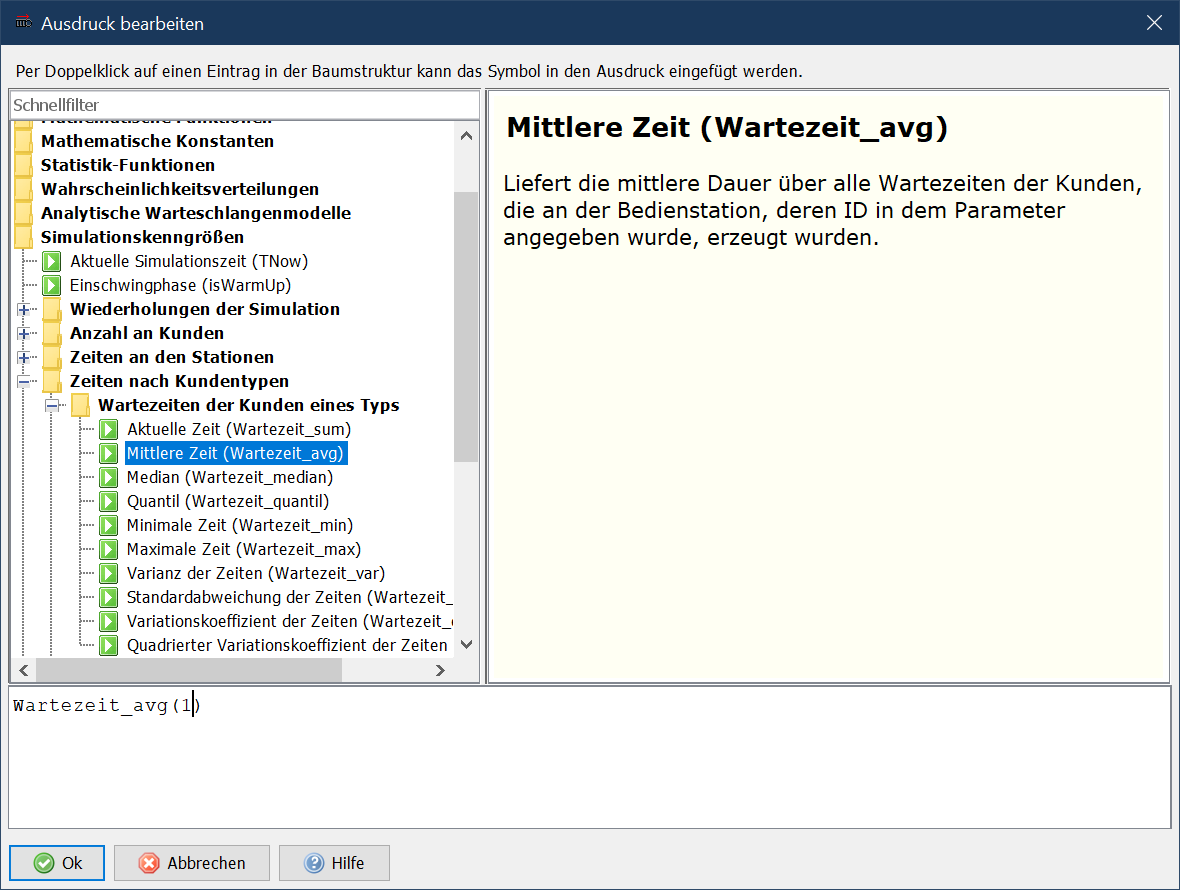
\includegraphics[width=14cm]{DialogExpressionBuilder.png}}
	\label{fig:ExpressionBuilder}
\end{figure}